\documentclass{article}
\usepackage[utf8]{inputenc}
\usepackage{pgfplots}
\usepackage{verbatim}
\pgfplotsset{width=0.8\textwidth,compat=1.16}
\usepackage{graphicx}
\graphicspath{ {./images/} }
\usepackage{float}
\usepackage{listings}
\usepackage{xcolor}

\definecolor{codegreen}{rgb}{0,0.6,0}
\definecolor{codegray}{rgb}{0.5,0.5,0.5}
\definecolor{codepurple}{rgb}{0.58,0,0.82}
\definecolor{backcolour}{rgb}{0.95,0.95,0.92}
\definecolor{black}{rgb}{0,0,0}
\lstdefinestyle{mystyle}{
    backgroundcolor=\color{backcolour},
    commentstyle=\color{codegreen},
    keywordstyle=\color{magenta},
    numberstyle=\tiny\color{codegray},
    stringstyle=\color{codepurple},
    basicstyle=\ttfamily\footnotesize,
    breakatwhitespace=false,
    breaklines=true,
    captionpos=b,
    keepspaces=true,
    numbers=left,
    numbersep=5pt,
    showspaces=false,
    showstringspaces=false,
    showtabs=false,
    tabsize=2
}

\lstset{style=mystyle}

\begin{document}
    \begin{titlepage}
    \begin{center}
        \vspace*{1cm}

        \huge
        \textbf{PVZ-Like}

        \vspace{0.5cm}

        \Large
        Final Report

        \vspace{4cm}

        \large
        \textbf{Paolo Penazzi} \\
        \textit{paolo.penazzi@studio.unibo.it} \\
        \textbf{Angelo Parrinello} \\
        \textit{angelo.parrinello@studio.unibo.it} \\
        \textbf{Francesco Foschini} \\
        \textit{francesco.foschini6@studio.unibo.it} \\
        \textbf{Davide Alpi} \\
        \textit{davide.alpi@studio.unibo.it} \\

        \vspace{4cm}

        \Large
        Paradigmi di Programmazione e Sviluppo\\
        M.S. Engineering and Computer Science\\
        Alma Mater Studiorum - University of Bologna\\
        Campus of Cesena\\
        Italy\\

    \end{center}
\end{titlepage}
    \tableofcontents
    \newpage
\section{Introduzione}
Il gruppo si è posto come obiettivo la realizzazione di una riproduzione di Plant VS Zombie:
gioco di strategia, appartenente alla famiglia \textit{Tower Defense}, nel quale il giocatore deve impedire ai nemici di attraversare un determinato percorso.

La difesa sarà organizzata attraverso il
posizionamento di torrette che attaccano in maniera automatica il nemico, secondo determinate regole.
In particolare, in PVZ i nemici sono rappresentati da ondate di Zombie di diverso tipo a difficoltà crescente,
da contrastare con il piazzamento delle piante: queste ultime dovranno impedire agli zombie di raggiungere l'abitazione.
Il piazzamento delle piante è limitato dal numero di risorse che il giocatore ha a disposizione.
Con il passare del tempo il giocatore aumenterà il numero di risorse disponibili.

\subsection{Linguaggio}
Alcuni termini che verranno utilizzati in seguito:
\begin{itemize}
    \item \textbf{Zombie}: qualsiasi tipo di nemico.
    \item \textbf{Pianta}: qualsiasi tipo di entità piazzata dal giocatore per difendersi.
    \item \textbf{Troop}: qualsiasi tipo di entità, può essere sia una pianta che uno zombie.
    \item \textbf{Bullet}: di vario tipo, vengono sparati sia dalla piante che dagli zombie.
    \item \textbf{Wave}: un'ondata di zombie.
\end{itemize}

    \newpage
\section{Processo di sviluppo}
\label{sec:development}
Il processo di sviluppo adottato dal team è ispirato a Scrum: sarà basato su \textbf{sprint} e \textbf{obiettivi}
per realizzare il progetto in maniera \textbf{agile}.
All'interno del team sono stati scelti un \textit{committente} e un \textit{product owner}.
Il team effettua sprint della durata di circa due settimane, durante i quali si definiscono gli obiettivi e si suddividono i compiti.
Di seguito, si discutono gli elementi fondamentali del processo di sviluppo adottato.

\subsection{Meeting}
I meeting sono un fattore fondamentale per il processo di sviluppo e avvengono con cadenza quasi giornaliera
e con durate differenti in base all'importanza. Vista la distanza tra i membri del
team (due in Svezia e due in Italia) la maggior parte degli incontri è avvenuta
utilizzando \textit{Microsoft Teams} come piattaforma principale.

\subsection{Modalità di divisione in itinere dei task}

\subsubsection{Definition of Done}
Una funzionalità di gioco viene definita completata quando, a seguito di una revisione da parte
di un altro componente del team, viene pubblicata sul \textit{branch} principale. Questa revisione può essere avvenuta
tramite \textit{pair-programming} oppure tramite il meccanismo di \textit{pull-request}.

\subsubsection{Coordinazione}
La comunicazione è fondamentale per un processo di sviluppo Agile, anche se i membri del team si conoscono a fondo.
Per coordinarsi al meglio, il team ha deciso di utilizzare \textbf{Trello},
con il quale vengono tracciati i task dei singoli membri con il rispettivo andamento,
individuando un flusso di lavoro all'interno di ogni sprint organizzativo.
Inoltre, il \textit{product owner} del team ha redatto un \textit{product backlog} nel
quale si è tenuto traccia dei task, indicando
per ciascuno il grado di difficoltà di progettazione e/o implementazione e l'effort da esso richiesto in ciascuno sprint.

\subsubsection{Meeting iniziale}
Prima della proposta del progetto, è avvenuto un incontro all'interno del quale sono stati decisi i seguenti fattori essenziali:
\begin{itemize}
    \item \textbf{Ruoli}: è stato scelto il product owner (Paolo Penazzi) e il committente (Angelo Parrinello).
    \item \textbf{Specifiche}: sono stati decisi gli obiettivi funzionali, facendo attenzione alla loro fattibilità.
    \item \textbf{Primo Sprint}: è stata decisa l'organizzazione del primo sprint, definendo l'obiettivo finale e suddividendo dei task tra i componenti del gruppo.
\end{itemize}
La durata del primo meeting è stata di circa 2 ore.

\subsubsection{Sprint Planning}
All'inizio di ogni sprint viene effettuato un incontro all'interno del quale si discutono i
risultati dello sprint precedente e si definiscono gli obiettivi di quello successivo.
I principali punti sui cui ci si focalizza sono i seguenti:
\begin{itemize}
    \item Definizione degli obiettivi.
    \item Definizione ed assegnazione dei task.
    \item Valutazione dell'andamento complessivo del progetto, rimarcando eventuali ritardi.
    \item Valutazione dello sprint precedente.
\end{itemize}

La durata ideale degli sprint planning è fissata a 2 ore.

\subsubsection{Divisione dei compiti}
L'effettiva divisione dei compiti, da eseguire nello sprint successivo all'interno del team, viene fatta
contestualmente alla chiusura dello sprint precedente. La suddivisione dei compiti terrà conto del carico di lavoro, degli
impegni del singolo componente e dell'eventuale lavoro incompiuto dallo sprint precedente.

\subsection{Modalità di revisione in itinere dei task}

\subsubsection{Ridistribuzione del carico lavorativo}
All'interno dello sprint è previsto la ridistribuzione del lavoro. Infatti, se ci si accorge che il carico di lavoro
di un task risulta essere diverso da quello previsto riteniamo possibile ridefinire i partecipanti al suddetto task.
Questo bilanciamento dovrà avvenire al seguito di un \textit{Stand-up Meeting} e di una valutazione da parte dell'intero
gruppo.

\subsubsection{Stand-up Meeting}
Con cadenza quasi giornaliera, il team effettua degli incontri in cui ognuno dei membri
espone il lavoro portato a termine, dichiarando eventuali difficoltà.
La durata ideale degli stand-up meeting è fissata a 10/15 minuti.

\subsection{Tool Ausiliari}
A supporto del processo agile, il team si impone di utilizzare strumenti con lo scopo di migliorare
l’efficienza e di consentire al gruppo di concentrarsi maggiormente sul processo di sviluppo.

\subsubsection{Automazione}
Sono stati adoperati i seguenti processi:
\begin{itemize}
    \item \textbf{Test Driven Development} - scrivere in anticipo dei test per il proprio codice,
    permette di intercettare eventuali errori che insorgono durante l'integrazione del lavoro reciproco.
    \item \textbf{Continuous Integration} - per verificare la compatibilità e la correttezza del software prodotto
    viene sfruttata la funzionalità \textbf{GitHub Actions}, definendo all'inizio del processo di sviluppo un
    preciso workflow che assicura la corretta manutenzione del progetto.
    \item \textbf{Continuous Delivery} - per evitare di produrre manualmente gli \textit{artifacts}
    alla fine di ogni Sprint, è stato individuato un workflow adatto che permettesse di creare delle
    release automatiche ogni qual volta il branch \textit{release} di git venisse aggiornato.
    \item \textbf{Automatic Dependecies Updates} - per mantenere aggiornate le dipendenze del codice sorgente, attraverso
    delle pull request, verrà impiegato il bot \textbf{Renovate}.
    \item \textbf{Code Quality Automation} - attraverso il tool \textbf{Sonarcloud} sarà possibile automatizzare la ricerca
    di segnali di cattiva qualità del codice quali \textit{code repetition}, \textit{bugs} e \textit{vulnerabilità}.
\end{itemize}

\subsubsection{Versioning}
Per gestire in maniera ottimale il codice prodotto, si è deciso di impiegare \textbf{Git}, già utilizzato da tutti i componenti del gruppo. Il team adotterà \textbf{GitFlow} come flusso di lavoro, che prevede di avere due \textit{stable branch} (nel nostro caso \texttt{main} e \texttt{release}) e un branch per ogni feature in via di sviluppo. \\
Allo stato attuale, il gruppo non ha intenzione di adottare Semantic Versioning per le release.
Si ritiene però opportuno l'utilizzo dei \textit{Conventional Commits} per due motivi: i singoli commit saranno più chiari
e in futuro si potrebbe decidere di impiegare il Semantic Versioning. \\
Le release saranno effettuate al termine di ogni sprint. Ognuna di esse avrà un tag del tipo \textit{0.1.0} che incrementerà ad ogni rilascio.


    \newpage
\section{Requisiti}
\subsection{Business}
Il sistema dovrà emulare il gioco Plants Vs Zombies.
Sono stati individuati i seguenti requisiti di business:
\begin{itemize}
    \item Il gioco dovrà avere un menù di inizio e fine partita.
    \item Sarà possibile giocare una partita intera ad un clone di Plants Vs Zombies.
    \item Sarà possibile visualizzare il campo di gioco e interagire con esso.
\end{itemize}

\subsection{Funzionali}
Il gioco si compone di un insieme di entità e regole, per quanto riguarda gli elementi della partita:
\begin{itemize}
    \item Le entità in gioco possono essere di tre tipi:
    \begin{itemize}
        \item Zombie
        \item Piante
        \item Bullet
    \end{itemize}
    \item Il campo da gioco deve essere composto da più corsie.
    \item Il gioco sarà composto da tre schermate: menù iniziale, schermata di gioco e menù finale.
    \item I nemici avanzeranno lungo le corsie da destra verso sinistra.
    \item Ogni Zombie e ogni Pianta deve avere un campo visivo.
    \item Gli Zombie saranno organizzati in ondate.
    \item Le ondate contengono una serie di Zombie, la cui dimensione e complessità aumenta con l'avanzare del gioco.
    \item Quando uno Zombie si avvicina sufficientemente ad una Pianta, lo Zombie la attaccherà.
    \item Quando uno Zombie entra nel campo visivo di una Pianta, questa lo attaccherà.
    \item Se una Pianta o uno Zombie viene colpito, perderà vita.
    \item Se una Pianta o uno Zombie rimane senza vita, morirà e verra rimossa dal campo di gioco.
    \item Se uno Zombie raggiunge la fine della corsia, la partita termina.
    \item Ogni Pianta avrà un costo di piazzamento.
    \item Per piazzare una Pianta è necessario avere un numero di risorse maggiore o uguale al costo della Pianta.
    \item I tipi di Piante previsti sono:
    \begin{itemize}
        \item Peashooter: spara Bullet che colpiscono il primo Zombie che incontrano.
    \end{itemize}
    \item I tipi di zombie previsti sono:
    \begin{itemize}
        \item BasicZombie: quando in contra una pianta, la attacca.
    \end{itemize}
    \item I tipi di Bullet previsti sono:
    \begin{itemize}
        \item Peabullet: il Bullet sparato dal Peashooter.
        \item PawBullet: il Bullet sparato dal BasicZombie.
    \end{itemize}
\end{itemize}

\subsubsection{Utente}
L'utente deve poter:
\begin{itemize}
    \item Avviare una partita.
    \item Piazzare le Piante nelle celle libere del campo da gioco.
    \item Vedere le statistiche a fine partita e riavvare il gioco.
\end{itemize}

\subsubsection{Non Funzionali}
I requisiti non funzionali individuati per il progetto sono:
\begin{itemize}
    \item Realizzazione di software estendibile e rivisitabile.
    \item Realizzazione di un'esperienza di gioco godibile (usabilità, bilanciamento, qualità grafica).
    \item Il gioco deve rimanere fluido per un numero ragionevole di ondate.
\end{itemize}

\subsection{Opzionali}
Sono stati individuati dei requisiti non obbligatori del progetto ma che tuttavia accrescerebbero il valore del prodotto finale:
\begin{enumerate}
    \item Possibilità di mettere in pausa, riprendere e velocizzare il gioco.
    \item Aumentare i tipi di Piante.
    \item Aumentare i tipi di Zombie.
    \item Aumentare i tipi di Bullet.
    \item Implementazione di un meccanismo di gestione della difficoltà.
    \item Inserire delle animazioni.
    \item Inserire la possibilità di generare campi di gioco particolari.
\end{enumerate}

\subsection{Implementativi}
Il gioco verrà sviluppato in Scala e dipenderà da alcuni framework aggiuntivi quali libGDX, Akka e TuProlog.
Il software prodotto deve essere testato con ScalaTest per garantire la manutenzione, la qualità e la corretta integrazione del codice dei vari componenti del team.
    \newpage
\section{Architettura}

\subsection{Pattern Architetturale}
Il pattern architetturale scelto per questo progetto è il celebre \textbf{MVC}.
Questa scelta ha portato ad una divisione netta dei compiti tra i vari componenti. In fase di design il pattern si
è rivelato importante perchè ci ha permesso di dividere in maniera ottimale il flusso di lavoro e i task che ognuno dei
componenti doveva portare a termine. Questa scelta, unita al \textit{modello ad attori}, ha aiutato
lo sviluppo permettendoci di astrarre alcuni concetti e rendere il più indipendenti possibili i vari componenti del software.

\subsection{Modello ad Attori}
La presenza di un elevato numero di entità all’interno dell’applicazione ha portato alla luce
l’esigenza di gestire, già a livello architetturale, la possibilità di sfruttare a pieno la potenza
della cpu, rendendo quindi il programma concorrente. \\
In particolare, per astrarre dalla gestione
di problematiche tipiche di sistemi concorrenti (mutua eclusione e corse critiche) si è deciso di
adottare un approccio basato su attori.\\
Dal momento che ogni attore incapsula al suo interno
un flusso di controllo basato su \textit{event loop} e che le interazioni avvengono esclusivamente
attraverso scambio di messaggi, non è necessario gestire meccanismi di sincronizzazione. \\
Inoltre, abbiamo ritenuto il modello ad attori particolarmente adeguato per la realizzazione
dell’applicazione in quanto essi incapsulano il \textbf{comportamento}, delle entità all’interno del modello. \\
Per tali motivi si è deciso quindi di adottare il framework
\textit{Akka} per sviluppare in maniera semplificata il sistema ad attori.

\subsubsection{Vantaggi del Modello ad Attori}
Di seguito si analizzano i vantaggi dell'utilizzo di Akka:
\begin{itemize}
    \item Chiarezza del comportamento del sistema fin da subito.
    \item Espressività del codice relativo al comportamento delle entità di gioco.
    \item Migliore incapsulamento dei task di ogni componente.
    \item Sistema maggiormente modulare.
    \item Astrazione di meccanismi di concorrenza di basso livello (semafori, monitor, ecc.).
\end{itemize}

\subsubsection{Svantaggi del Modello ad Attori}
Alcune criticità dell'utilizzo di Akka sono le seguenti:
\begin{itemize}
    \item Difficoltà nel testing degli attori.
    \item Il numero dei messagi scambiati è proporzionale alla dimensione del sistema.
    \item Eventuale \textit{bottleneck} dovuto al message passing.
\end{itemize}

\subsection{Architettura Complessiva}
L'impiego del paradigma ad attori combinato al pattern architetturale MVC ci ha portato a modellare questi tre componenti
come essi stessi attori. Ognuno di essi gestisce messaggi di tipo diverso:
\begin{itemize}
    \item \textit{Command} - questo è il tipo di messaggio accettato dal GameLoop ovvero l'attore che fungerà da
    Controller del sistema. Questa tipologia di messaggi indica tutte le interazioni tra Controller, Model e View.
    \item \textit{ModelMessage} - questo è il tipo di messaggio accettato dagli attori del Model. I messaggi di questa categoria
    gestiranno l'avanzamento dello stato interno degli oggetti di Model.
    \item \textit{ViewMessage} - questo è il tipo di messaggio accettato dal ViewActor ovvero l'attore che fungerà da View
    del sistema. Questa serie di messaggi delineerà l'API per le interazioni tra View, Controller e utente finale.
\end{itemize}

\begin{figure}[H]
    \centering
    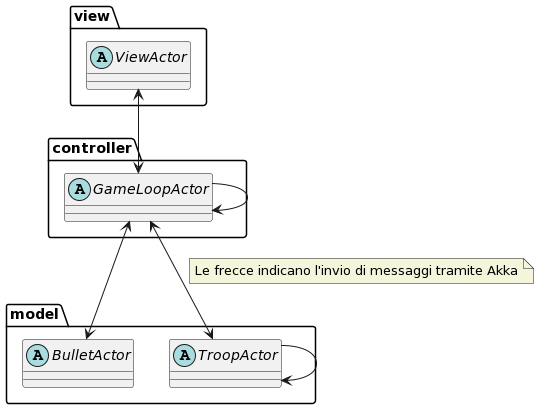
\includegraphics[width=\linewidth]{images/actor-architecture}
    \label{Diagramma delle classi dell'architettura complessiva.}
    \caption{Architettura finale dell'actor system.}
\end{figure}

È stato utilizzato il formalismo UML per modellare gli attori,
tuttavia, sono state adottate alcune convenzioni per facilitarne la compresione.
Le frecce rappresentato le interazione ad alto livello che avvengono tra i vari componenti.
Nonostante l'immagine  suggerisca la violazione del pattern MVC, le frecce rappresentano in realtà il flusso dei messaggi.
Per fare un esempio, gli attori del Model non inizieranno mai una relazione con il Controller,
bensì si limitano a rispondere ai messaggi che quest'ultimo spedisce.
    \newpage
\section{Design di Dettaglio}
Dopo aver analizzato l'architettura generale del sistema, in questa sezione viene effettuato uno studio sul design
di dettaglio del progetto.
Verranno evidenziati aspetti interni ai componenti, senza toccarne la reale implementazione.

\subsection{Design del Model}
E' stato creato un \textit{Trait} che modella tutte le entità del gioco come \textbf{Entity}. Questo tratto rappresenterà
alcuni degli aspetti fondamentali di ogni oggetto in gioco, ad esempio la posizione. Partendo da ciò sono stati definiti
altri due macro concetti fondamentali del nostro gioco:
\begin{itemize}
    \item \textbf{MovingAbility} - rappresenta l'abilità di movimento da parte delle entità.
    \item \textbf{AttackingAbility} - rappresenta l'abilità di un componente di gioco di attaccare un'altra entità.
\end{itemize}
\begin{figure}[H]
    \centering
    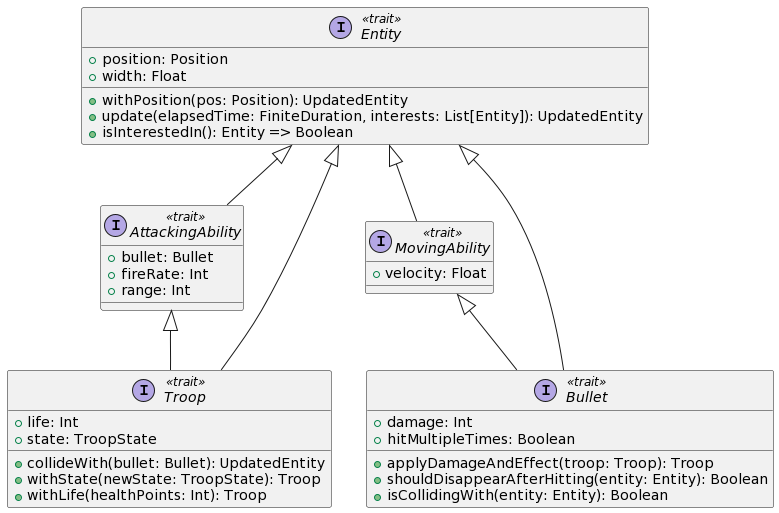
\includegraphics[width=\linewidth]{images/model-desing}
    \caption{Diagramma delle classi della gerarchia delle entità di gioco.}
\end{figure}
Attraverso queste due abilità abbiamo composto le altre entità base del gioco:
\begin{itemize}
    \item \textbf{Troop} - il trait \textit{Troop} modella tutta le entità di gioco che sono Piante o Zombie.
    \item \textbf{Bullet} - il trait \textit{Bullet} rappresenta le entità che vengono generate dalle Troop quando
    attaccano.
\end{itemize}
Ogni entità appena descritta presenta una controparte
reattiva, ovvero un attore, che si occupa del corretto aggiornamento della stessa e delle sue
interazioni all’interno del dominio.\\

La posizione delle entità è definita dal numero della corsia in cui si trova (y) e dal punto nella corsia nella quale si trova (x).\\

Le Troop incorporano un concetto di stato, che rispecchia la loro condizione attuale all'interno del gioco. Questi stati sono:
\begin{itemize}
    \item \textit{Idle}: la truppa non fa nulla, aspetta che avvenga qualcosa.
    \item \textit{Moving}: la truppa è in movimento.
    \item \textit{Attacking}: la truppa sta attaccando.
    \item \textit{Dead}: la truppa è morta.
\end{itemize}

\begin{figure}[H]
    \centering
    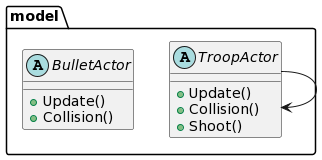
\includegraphics[width=0.61\linewidth]{images/detail-model.png}
    \caption{Messaggi degli attori Model.}
\end{figure}

\newpage

\subsection{Design della View}
La view, come standard da paradigma MVC, deve inoltrare al controller le richieste da parte dell'utente,
come il piazzamento delle piante.
Deve inoltre fornire API per renderizzare gli elementi del gioco (entità e metadata).

\begin{figure}[H]
    \centering
    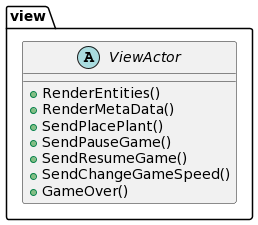
\includegraphics[width=0.61\linewidth]{images/detail-view.png}
    \caption{Messaggi del ViewActor.}
\end{figure}

\subsection{Design del Controller}
Per modularizzare al meglio il sistema e rispettare il \textit{Single Responsibility Principle}
sono stati introdotto degli attori che si occupano di controllare specifiche parti di sistema. Con questo presupposto sono
stati identificati cinque attori:
\begin{itemize}
    \item \textbf{RootActor} - attore \textit{Launcher} del sistema. Si occuperà di
    istanziare gli attori relativi alla View e al Loop del gioco.
    \item \textbf{GameLoopActor} - attore relativo al \textit{Loop} di gioco nonché
    \textit{Main Controller}. Tutti gli aggiornamenti di gioco saranno di sua responsabilità.
    \item \textbf{ViewActor} - attore relativo alla \textit{View} di gioco.
    La sua funzione sarà quella di renderizzare a schermo le informazioni relative al dominio.
    \item \textbf{BulletActor} - attore che incapsula il flusso di controllo di un singolo \textit{Bullet}.
    \item \textbf{TroopActor} - attore che incapsula il flusso di controllo di un singola \textit{Troop}.
\end{itemize}
In particolare si è voluto modellare gli attori relativi ai Bullet, Troop e
View in modo tale da avere esposti al Main
Controller solo determinate funzionalità a lui interessate.
Così facendo questi tre attori non fanno altro che rispondere
in maniera reattiva alle richieste del Controller ed inoltre permettono,
attraverso un'interfaccia più semplice, l'accesso
agli oggetti del Model che contengono un'interfaccia ben più complessa.
Questo design è tratto dal pattern \textbf{Facade}.

\begin{figure}[H]
    \centering
    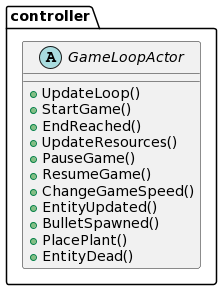
\includegraphics[width=0.61\linewidth]{images/detail-controller.png}
    \caption{Messaggi degli attori Controller.}
\end{figure}




    \newpage
\section{Implementazione}
Analizziamo ora gli aspettivi implementativi del sistema. Per
riflettere la suddivisione del lavoro durante il processo di sviluppo, questa sezione presenta
una parte descrittiva per ognuno dei membri del team.

\subsection{Paolo Penazzi}
Il mio compito all’interno del progetto è stato quello di modellare la gerarchia di Entity e Troop,
implementare le piante e l'attore che ne definisce il comportamento, realizzare i proiettili relativi alle piante e di generare le wave insieme a Parrinello.

\subsubsection{Troop}
Durante la modellazione delle Entity, insieme agli altri membri del gruppo è stato notato che il comportamento in comune tra le piante e gli zombie poteva essere definito in un concetto di Troop.

Grazie ai \textbf{mixin} mi è stato possibile definire il \texttt{trait Troop} come estensione del \texttt{trait Entity}
a cui viene aggiunta l'abilità di attaccare \texttt{AttackingAbility}.
Questo nuovo concetto di \texttt{Troop} ci ha permesso, in tutto il progetto, di trattare le piante e gli zombie allo stesso modo.

Durante l'analisi del dominio ho notato che le entità subiscono spesso modifiche durante la partita: l'aggiornamento della posizione, quello della vita o quello dello stato.
Ho quindi cercato un modo per rendere naturale questa modifica, che rispettasse però due vincoli:
\begin{itemize}
    \item Le entità devono essere immutabili.
    \item L'aggiornamento deve essere fatto in maniera funzionale.
\end{itemize}
Dopo vari tentativi con approcci differenti, la scelta è ricaduta sulla definizione di un metodo per ogni caratteristica da modificare: tale metodo prenderà in input il nuovo valore e restituirà una nuova troop con il campo aggiornato.

Questi metodi sono stati implementati utilizzando il metodo \textbf{copy} di Scala, che permette di fare proprio ciò di cui avevo bisogno.
L'unico difetto di questa soluzione è che il metodo \textit{copy} è disponibile sono nelle \textbf{case class}, quindi tutte le classi che estendono \textit{Troop} dovranno implementare quei metodi.

A questo punto la modifica di una troop può essere effettuata utilizzando la \textbf{notazione infissa}:

\begin{lstlisting}[language=Scala, label=code:troop-update, caption= Aggiornamento di una troop.]
    val troop: Troop
    val updatedTroop = troop withLife 50 withPosition (0,0)
\end{lstlisting}

Questa soluzione è stata poi adottata anche nei Bullet.

Gli stessi principi mi hanno guidato nella creazione di un modo di creare le troop che fosse il più funzionale possibile.
Ho quindi rivisitato il \textbf{pattern builder} per creare troop di qualsiasi tipo: ho creato un \texttt{trait TroopBuilder}
con un unico metodo \textit{build} che ritorna la troop desiderata.
Utilizzando le \textbf{given conversion} ho definito, per ogni possibile tipo di Troop, un'istanza del builder che si occupa
della creazione di quest'ultima.
Per rendere il builder più coerente con il linguaggio del progetto ho definito un metodo \textit{ofType} che che dato un tipo
di troop utilizza il builder per restituire la nuova entità.

\begin{lstlisting}[language=Scala, label=code:troop-builder, caption= Builder per la creazione di una Troop.]
    object Troops:
        trait TroopBuilder[T <: Troop, B <: Bullet]:
            def build: T

        given TroopBuilder[BasicZombie, Bullet] with
            override def build: BasicZombie = BasicZombie()

        given TroopBuilder[Wallnut, Bullet] with
            override def build: Wallnut = Wallnut()

        def ofType[T <: Troop](using troopBuilder: TroopBuilder[T, Bullet]): T =
            troopBuilder.build
\end{lstlisting}

Tutto ciò rende più funzionale la creazione di una troop, che può essere effettuata in questo modo:

\begin{lstlisting}[language=Scala, label=troop-creation, caption=Troop creation. ]
    val troop: Troop = Troops.ofType[BasicZombie]
\end{lstlisting}

L'idea di avere un builder per creare le entità del model è piaciuta al team, per questo ho implementato un secondo builder per creare \textit{Bullet}.
Non entrerò nel dettaglio in quanto per implementarlo, ho seguito il modello del \textit{TroopBuilder}.

\subsubsection{TroopActor}
Avendo adottato un'architettura ad attori, ogni troop, in fase di creazione, viene associata ad un attore che ne definisce il comportamento.
Il TroopActor ha un solo Behaviour e non è mai proattivo: risponde solamente ai messaggi ricevuti dal GameLoop, rispettando il pattern \textbf{MVC}.

Il punto di forza di questo \textit{Troop Actor} è che modella il comportamento delle piante e degli zombie come se fossero equivalenti.
Questo conferma le scelte di design fatte, in particolare quella di creare un \textit{trait troop} comune sia alle piante che agli zombie.

Ad ogni iterazione del GameLoop il TroopActor riceve un messaggio di \textit{Update()} a seguito del quale:
\begin{itemize}
    \item Aggiorna la propria troop.
    \item Se la troop ha raggiunto la fine della corsia notifica il GameLoop.
    \item Manda la troop aggiornata al GameLoop.
    \item Se c'è un nemico attaccabile, manda a se stesso un messaggio Shoot().
    \item Ricrea il proprio Behaviour con la troop aggiornata.
\end{itemize}

Nel caso ci sia un'entità da attaccare, riceverà il messaggio Shoot(), che si è precedentemente inviato, a seguito del quale:

\begin{itemize}
    \item Crea il bullet che la propria troop spara.
    \item Crea un BulletActor che controlla il bullet.
    \item Notifica il GameLoop dell'avvenuta creazione inviandogli il messaggio BulletSpawned(), contenente il riferimento al bullet e al BulletActor.
\end{itemize}

Nel caso la troop venga colpita da un bullet, il TroopActor viene notificato dal GameLoop con il messaggio Collision(), a seguito del quale:

\begin{itemize}
    \item Applica il danno e l'eventuale effetto del bullet alla troop.
    \item Se la troop viene uccisa, risponde con il messaggio EntityDead()
    \item Se la troop non viene uccisa, risponde con il messaggio EntityUpdated()
\end{itemize}

Il comportamento del TroopActor viene mostrato nel seguente diagramma:

\begin{figure}[H]
    \centering
    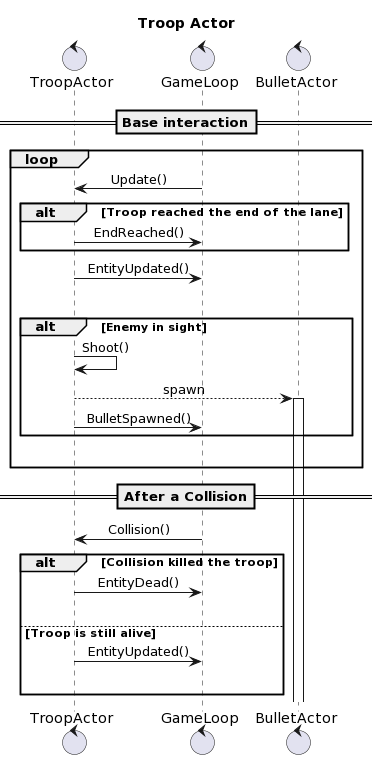
\includegraphics[width=0.8\linewidth]{images/troop-actor.png}
    \label{Diagramma di sequenza del Troop Actor.}
\end{figure}

\subsubsection{Plant}
Un'altra parte fondamentale del mio lavoro è stata la creazione dei vari tipi di piante: sono partito definendo un \texttt{trait Plant} che estende \textit{Troop} e modella il comportamento comune tra le varie piante.
Ho poi creato vari tipi di piante creando delle classi che estendono \textit{Plant}.

Durante l'implementazione di queste classi, ho notato che tutte le piante che sparano hanno lo stesso comportamente, l'unica cosa che cambia è il bullet che sparano.
Ogni tipo di pianta che spara può essere quindi identificata dal rispettivo bullet.

Ho cercato di migliorare la mia implementazione, provando a renderla il più riusabile possibile per non ripetere codice: ho tentato vari approcci, dall'utilizzo di classi astratte alla delegazione, ognuno dei quali presentava vantaggi e svantaggi.
La scelta finale è ricaduta sull'utilizzo di una \textbf{type class} che modella le piante che sparano.

Ho creato la classe \textit{Shooter} che è una type class generica sul tipo di bullet che spara.
Questa implementazione è stata possibile grazie all'utilizzo, nel \textit{trait Plant}, di un \textbf{abstract type} \textit{BulletType \textless: Bullet} per definire il tipo di ritorno del metodo \textit{bullet}.

\begin{lstlisting}[language=Scala, label=code:plant-shooter caption=Type class Shooter.]
case class Shooter[B <: Bullet]
    (bulletInstance: B,
    override val position: Position = (0, 0),
    override val life: Int = shooterDefaultLife,
    override val state: TroopState = defaultPlantState)
    extends Plant :

  override type BulletType = B
\end{lstlisting}

Per istanziare questa pianta ho definito un metodo ad-hoc, che sotto utilizza il \textit{TroopBuilder} definito in precedenza.
È quindi possibile creare shooter nella seguente maniera:

\begin{lstlisting}[language=Scala, label=shooter-builder, caption=Shooter creation. ]
    val plant: Plant = Troops.shooterOf[PeaBullet]
\end{lstlisting}

In questa classe non rientrano due tipi di piante, il \texttt{wallnut} e la \texttt{cherry bomb}.
Queste sono state implementate utilizzando classi ad-hoc perchè hanno un comportamente diverso rispetto alle piante che sparano:
\begin{itemize}
    \item Il Wallnut è una pianta con tanta vita che però non può attaccare.
    \item La Cherrybomb è una pianta che quando piazzata esplode, colpendo tutti i tipi di \textit{Troop}.
\end{itemize}

Tutti i valori relativi alle piante (defaultLife, bullet, etc..) sono stati inseriti in un oggetto \texttt{PlantDefaultValues},
in modo da rendere più pulito il codice e facilitare il bilanciamento del gioco.

\begin{lstlisting}[language=Scala, label=default-values, caption=Plant default values.]
      val shooterDefaultLife: Int = 100
      val wallnutDefaultLife: Int = 150

      val bullets: Plant => PlantBullet =
        case s: Shooter[_] =>
        s.bulletInstance match
          case _: PeaBullet => Bullets.ofType[PeaBullet]
          case _: SnowBullet => Bullets.ofType[SnowBullet]
        case c: CherryBomb => CherryBullet(c.position)
\end{lstlisting}

Il diagramma della gerarchia delle piante è il seguente:

\begin{figure}[H]
    \centering
    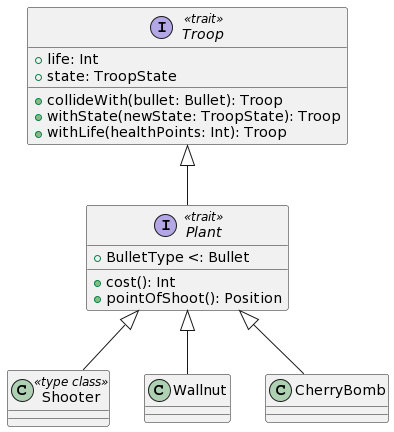
\includegraphics[width=0.8\linewidth]{images/plants.png}
    \label{Diagramma delle classi delle piante.}
\end{figure}

A seguito del mio lavoro sulle piante ho anche implementato i bullet relativi e contribuito, in maniera significativa, alla modellazione di questi ultimi.

\subsection{Angelo Parrinello}
Il mio compito all’interno del progetto è stato quello di modellare il \texttt{GameLoop}, le statistiche della partita ed infine mi sono occupato delle \texttt{Wave} (ondate di nemici) insieme a Penazzi. Inoltre, ho provveduto a sviluppare componenti di \texttt{Model} gestiti dal \texttt{GameLoop} quali \texttt{MetaData} e \texttt{GameData}, che si occupano rispettivamente della gestione di dati trasversali alla partita e di manipolare le entità in gioco. Infine, ho collaborato a stretto contatto con il team per implementare aspetti e funzionalità comuni di \texttt{Model}, \texttt{Controller} e \texttt{View}.

\subsubsection{GameLoop}
Il \texttt{GameLoop} è il componente che si occupa di aggiornare il \texttt{Model} e il successivo \textit{refresh} della \texttt{View}. Nel nostro contesto, il \texttt{GameLoop} si occupa anche di aggiornare il \texttt{Model} a seguito di una richiesta da parte dell'utente (es: piazzare una nuova torretta).\\
\\La funzione principale è quella di \textit{Update} del sistema. Tipicamente questo avviene attraverso un ciclo che richiama rispettivamente l'aggiornamento del \texttt{Model} e della \texttt{View}. Nel paradigma ad attori questo comportamento non è ammissibile in quanto si andrebbe a creare un \textit{handler bloccante}, bloccando il \textit{flusso interno} di controllo, facendo perdere reattività all'attore. L'attore emula questa comportamento utilizzando i \texttt{TimerScheduler} proprietari di \textit{Akka}: allo scadere di questo timer, l'attore invia un messaggio a sè stesso di tipo \texttt{UpdateLoop} ed infine ricrea il timer con un certo \textit{delay}. Il \texttt{GameLoop} alla ricezione della richiesta di aggiornamento, notifica gli attori del \texttt{Model} ed, in seguito alla risposta di quest'ultimi, aggiornerà la \texttt{View} con i dati rivisti. Di seguito viene schematizzato tale comportamento.

\begin{figure}[H]
    \centering
    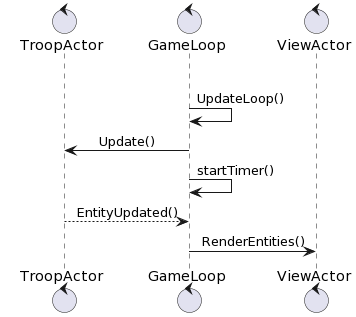
\includegraphics[width=0.61\linewidth]{images/game-update.png}
    \caption{Diagramma di sequenza della fase di Update del gioco.}
\end{figure}
Non entrerò nel dettaglio di altre sequenze di sistema che comprendono il \texttt{GameLoop} essendo abbastanza intuitive o che sono state implementata seguendo scelte già fatte (es: la fase di \textit{Update} delle risorse/soli del gioco che utilizza la stessa logica legata al \texttt{TimerScheduler}).\\

Il design del gioco assume che solo il \texttt{GameLoop} abbia coscienza dello stato intero del gioco, quindi esclusivamente lui conterrà tutte le informazioni ad esso associate. Una di queste è la \textit{sequenza} di entità, in un prefissato momento, nel gioco e la corrispondente parte reattiva. Durante lo sviluppo mi son reso conto che utilizzare delle semplici sequenze di \textit{tuple} non era l'ideale. Il codice risultante presentava diversi difetti quali \textit{ripetitività} e \textit{opacità}. Dopo aver vagliato diverse ipotesi, ho creato una \textbf{case class} che racchiudesse le informazioni relative al \texttt{Model} di un'entità e il riferimento al suo attore (chiamata \texttt{GameEntity} e \textbf{generica} in un sottotipo di \texttt{Entity}). In seguito, decisi di sfruttare il pattern funzionale \textbf{Pimp-my-library} convertendo le \texttt{Seq} in \texttt{GameSeq} (sequenze di \texttt{GameEntity}) con una \textbf{given conversion}.

\begin{lstlisting}[language=Scala, label=code:gamedata, caption=Parte del GameSeq.]
    given Conversion[Seq[GameEntity[Entity]], GameSeq] = 
        GameSeqImpl(_)

    /** Defines a [[GameSeq]] ... */
    trait GameSeq:
      /** Creates a [[Seq]] ... */
      def of[E <: Entity : GameSelectorBuilder]: Seq[GameEntity[E]] 
      = seq.collect(summon[GameSelectorBuilder[E]].by)

      /** Deletes a [[GameEntity]] ... */
      @targetName("delete")
      def :-(ref: ActorRef[ModelMessage]): Seq[GameEntity[Entity]] 
      = seq filter (_.ref != ref)
\end{lstlisting}

Questa scelta mi ha poi portato a creare un mini-\textbf{DSL} per creare in maniera elegante e funzionale sequenze di \texttt{GameEntity} definendo solo il tipo. L'idea di base dietro l'implementazione era avere \textbf{strategy} che definisse come una sequenza di \texttt{GameEntity} dovesse venire filtrata in base ad un tipo definito in input. Questo concetto, largamente sfruttato nella programmazione ad oggetti, vede un'analogia funzionale e idiomatica nei \textbf{contex-bounds}. Il metodo \texttt{of}, partendo dalla sequenza iniziale e sfruttando le \textbf{given instances}, genera così una nuova sequenza con solo gli elementi del tipo prestabilito.

\begin{lstlisting}[language=Scala, label=code:gameselector, caption= Creazione di una sequenza di gioco di soli tipi Troop.]
def of[E <: Entity : GameSelectorBuilder]: Seq[GameEntity[E]] =
    seq.collect(summon[GameSelectorBuilder[E]].by) 
    .
    .
 /** Contains some ways of creating [[GameSeq]]. */
  object GameSelector:
    /** Filters the [[GameEntity]] whose type is [[E]].
     *
     * @tparam E the type to filter.
     */
    trait GameSelectorBuilder[E <: Entity]:
      def by: PartialFunction[GameEntity[Entity], GameEntity[E]]

    given GameSelectorBuilder[Troop] with
      override def by: PartialFunction[GameEntity[Entity],               GameEntity[Troop]] = {
            case e if e.entity.isInstanceOf[Troop] => 
                GameEntity(e.ref, e.entity.asInstanceOf[Troop])
            }
\end{lstlisting}




Infine, il mio lavoro sul \texttt{GameLoop} mi ha portato ad introdurre il concetto di \textit{Collision}, di \textit{MetaData} e ad un utility object con funzionalità cardine per il controller di gioco. Nel caso delle collisioni, è stato interessante escogitare un metodo per rendere queste le più astratte possibili. In fase di modellazione mi è tornato utile il concetto delle \textbf{abstract types}. Infatti, in un primo momento sapevo che le collisioni sarebbero avvenuti tra due oggetti di tipo anche diverso, ma non erano stati definiti. Così facendo, le specifiche collisioni (al momento solo una) potranno essere definite più avanti nel tempo. Sempre rimanendo in tema collisioni, un altro punto importante è stato cercare una maniera \textit{idiomatica} e più \textit{funzionale} possibile per controllare in un'unico passaggio tutte le collisioni in un dato istante; \texttt{checkCollision} era stato implementato inizialmente con una serie di \textit{foreach}, \textit{map} e \textit{flatmap} ma, durante lo sviluppo, mi accorsi che così facendo il codice diveniva \textit{oscuro} ad un primo sgaurdo, più difficile da elaborare ed \textit{error-prone}. La scelta è quindi ricaduta sull'utilizzo di una \textbf{for-comprehension}, che aggiungendo lo \textit{zucchero sintattico} necessario, rendeva il tutto più chiaro e fluente.

\begin{lstlisting}[language=Scala, label=code:checkcollision, caption= Metodo che controlla e crea le collisioni.]
/** Detects [[Collision]] ... */
  def checkCollision(entities: Seq[GameEntity[Entity]]): 
    Seq[BulletTroopCollision] =
        for
            b <- entities.of[Bullet]
        yield
            BulletTroopCollision(b, for
                e <- entities.of[Troop]
                if b.entity isCollidingWith e.entity
            yield e)
\end{lstlisting}







\subsubsection{Statistiche}
Le \textit{Statistiche} sono quelle informazioni importanti per l'utente riguardo la partita appena svolta. Questi dati sono raccolti man mano che la partita avanza, tramite il \texttt{GameLoop}. In principio, sono stati definite quali statistiche andassero create. In generale, si è convenuto che le tre macro-tematiche dovessero essere: informazioni generali (es: numero di rounds) e informazioni su \texttt{Plant}/\texttt{Zombie} (es: numero di zombie uccisi). Quindi, ho ragionato su come il \texttt{GameLoop} dovesse manutenerle e in quali occasioni andassero aggiornate. Questo secondo step mi ha fatto capire che la struttura delle statistiche, così come quella dei \texttt{MetaData}, dovesse essere del tutto \textbf{immutabile}. Un uso sistematico di oggetti immutabili porta a codice più \textit{comprensibile} ed a facilitare la fase di \textit{debugging}. In fase implementativa, sono stati create tre \textit{Traits} ognuno con un compito specifico:
\begin{itemize}
    \item \texttt{GameStats}: definisce le informazioni di carattere generale sul gioco;
    \item \texttt{ZombieStatsOps}: definisce delle informazioni specifiche agli \texttt{Zombie};
    \item \texttt{PlantStatsOps}: definisce delle informazioni specifiche alle \texttt{Plant}.
\end{itemize}
Il concetto appena descritto era perfettamente adattabile al contesto dei \textbf{self-types} e \textbf{mixins}: concettualmente infatti è corretto che le informazioni relative agli \texttt{Zombie}/\texttt{Plant} venissero derivate solo utilizzando i dati generali. Inoltre, è possibile ottenere una sorta di ereditarietà (ma senza i problemi ad esso legati) e rappresentare questi concetti come \textit{decorazioni} componibili.

\begin{lstlisting}[language=Scala, label=code:statistics, caption=Statistiche relative agli Zombie.]
  /**
   * Defines which [[Zombie]]'s insights we want to gather from the game.
   */
  trait ZombieStatsOps:
    stats: GameStats =>
    /**
     *
     * @return the [[Zombie]]s killed.
     */
    def getZombies: Seq[Zombie] =
      stats.entities.foldLeft(List.empty)((acc, e) => e match {
        case zombie: Zombie => acc :+ zombie
        case _ => acc
      })
\end{lstlisting}



\subsubsection{Wave}
La parte che sono in procinto di spiegare, è stata modellata e sviluppata in modalità di \textbf{pair-programming} con il collega Penazzi Paolo. Per ragioni di impaginazione abbiamo deciso di inserirla sotto la mia sezione implementativa.\\

La \texttt{Wave} è una sequenza prestabilita di \textit{Zombie}. Le partite sono organizzate a \texttt{Wave}, che scandiscono il ciclo di vita del gioco. All'interno di una \texttt{Wave} possono essere presenti tutti i tipi di \texttt{Zombie} definiti nel gioco. I tipi e il numero degli \texttt{Zombie} che compongono la \texttt{Wave} determina la \textit{potenza} di quest'ultima. Con l'avanzare del gioco le \texttt{Wave} avranno una potenza sempre maggiore: comportamento incrementale tipico dei \textit{tower defense}. E' stato creato un oggetto \texttt{WaveGenerator} incaricato di generare le ondate di \texttt{Zombie}. Le ondate di \texttt{Zombie} possono essere generate in due modi:
\begin{itemize}
    \item Utilizzando \textbf{Scala}: in questa maniera si genera un'ondata di zombie composta solo da \texttt{BasicZombie}. L'ondata viene creata attraverso una funzione \textbf{tail recursive}.
    \begin{lstlisting}[language=Scala, label=code:tailrec-basiczombie, caption=Tail recursive Function per la creazione di Wave con Scala.]
  @tailrec
  private def createEnemyList(n: Int)(l: Seq[Zombie]): Seq[Zombie] =
    n match
      case 0 => l
      case _ => createEnemyList(n - 1)(l = l :+ BasicZombie())
\end{lstlisting}
    \item Utilizzando \textbf{Prolog}: in questa maniera si genera un'ondata di \texttt{Zombie} composta da qualsiasi tipo di nemico. Il processo sfrutta il \texttt{TuProlog Engine} per creare sequenze di tipi di \texttt{Zombie} casuali ma che rispecchino la potenza dell'ondata.
    \begin{lstlisting}[language=Prolog, label=code:prolog-theory, caption=Prolog Theory.]
% wave/2(+WavePower, -ListOfZombies)
% Returns a wave of zombies of the given power.
wave(0, []):- !.
wave(1, [1]):- !.
wave(2, [X|L]) :- random_zombie(2, X), M is 2 - X, wave(M, L), !.
wave(N, [X|L]) :- N > 2, random_zombie(3, X), M is N - X, wave(M, L).

% random_zombie/2(+MaxValue, -RandomNumber)
% Returns a RandomNumber between 1 and MaxValue.
% In this game each number is associated to a zombie.
random_zombie(Max, X) :- rand_int(Max, N), X is N + 1.
\end{lstlisting}
    Il predicato \texttt{random\_zombie} si occupa di generare un numero casuale fra uno e \texttt{Max} il quale corrisponde ad un tipo di \texttt{Zombie}. Il predicato \texttt{wave}, data una potenza \texttt{WavePower} ritornerà una tra tutte le possibili sequenze di \texttt{Zombie} di tale potenza.\\

    Per agevolare il processo realizzativo delle \texttt{Wave} e per integrare in maniera più fluente \texttt{TuProlog}, è stato messo a disposizione un metodo per generare \texttt{Wave} che utilizza al suo interno un engine per risolvere le \textit{query} in input.

    \begin{lstlisting}[language=Scala, label=code:prolog-engine, caption=Integrazione del Prolog Engine.]
    /** Implementations of [[Engine]]... */
    case class PrologEngine(theory: Theory) extends Engine:
      val engine: Prolog = new Prolog
      engine.setTheory(theory)

      override def generateWave(power: Int): List[Zombie] =
        import WaveTerm.given
        val query: String = "wave(" + power + ", L)"
        val solution: LazyList[SolveInfo] = solve(query)
        PrologSolution.waveFromPrologSolution(solution.head)

      override def solve: Term => LazyList[SolveInfo] = 
        term => LazyList.continually(engine solve term)
\end{lstlisting}




    La soluzione così fornita però risultava inutilizzabile. E' stato necessario quindi definirsi dei metodi utili in fase di ricostruzione del risultato finale ossia la sequenza di \texttt{Zombie}. Per riuscire ad ottenere l'ondata finale, il il risultato dell'\texttt{PrologEngine} viene \textit{parsato}, sostituendo i numeri all'interno della soluzione con i rispetti \texttt{Zombie}. Lo stesso principio delle \textbf{given conversion}, come si può notare dal listato sotto, è stato impiegato molteplici volte all'interno della classe per favorire \textit{idiomaticità} e \textit{comprensibilità} oltre che per fornire un \textbf{adapter} automatico che non introducesse \textit{boilerplate code} inutile.

    \begin{lstlisting}[language=Scala, label=code:prolog-solution, caption=Oggetto di utility per deserializzare le soluzioni TuProlog.]    
  /** Contains useful method for deserializing TuProlog solutions. */
  object PrologSolution:
    given Conversion[SolveInfo, List[Zombie]] =
        e => waveFromTerm(e.getTerm("L"))

    private def waveFromTerm(term: Term): List[Zombie] =
      term.toString.replaceAll("\\[|\\]", "")
        .split(",")
        .foldRight(List.empty[Int])((e, acc) 
            => acc :+ e.toInt)
        .map(powerToZombie(_))
\end{lstlisting}




\end{itemize}
\subsection{Francesco Foschini}
Il mio compito all'interno del progetto, è stato quello di modellare la gerarchia di \texttt{Entity} del gioco.
In particolare mi sono occupato della implementazione del model degli zombie, dei proiettili e l'attore che definisce il comportamento dei proiettili.
Ho partecipato inoltre allo sviluppo del \texttt{Troop Actor} del \texttt{Menù Screen} e del \texttt{Game Screen}.

\subsubsection{Bullet}
I proiettili rappresentano all'interno del gioco l'attacco delle \texttt{Plant} e degli \texttt{Zombie}.\\

Grazie alla buona gerarchia di caratteristiche definite in \texttt{Entity}, è stato possibile grazie  ai \textbf{mixins},
dotare il trait \texttt{Bullet} dell'abilità di movimento \texttt{Movement Ability}.
Il trait \texttt{Bullet} rappresenta quindi l'entità base "sparata" da una \texttt{Troop}.
Tutti i \texttt{Bullet} presentano un comportamento comune: hanno una posizione, una velocità, una dimensione ed un danno.\\


Successivamente sono stati individuati due diversi sottotipi\\ \texttt{Bullet}: \texttt{ZombieBullet} e \texttt{PlantBullet}.
Il primo è il trait che modella il colpo base degli \texttt{Zombie} mentre il secondo si riferisce all'attacco base delle \texttt{Plant}.

Attraverso il metodo \texttt{checkCollision} i \texttt{PlantBullet} possono collidere solamente contro le entità di tipo \texttt{Zombie} mentre,
al contrario, gli \texttt{ZombieBullet} potranno colpire solamente le entità sottotipo di \texttt{Plant}.

Mi sono successivamente concentrato nell'implementazione di due tipi di \texttt{ZombieBullet}: \texttt{PawBullet} (il bullet dei
\texttt{BasicZombie} e \texttt{FastZombie}) e lo \\
\texttt{SwordBullet} (il bullet dei \texttt{WarriorZombie}).
Lo \texttt{SwordBullet} è un attacco più potente rispetto al \texttt{PawBullet}.\\

Volendo seguire un approccio puramente funzionale, favorendo l'immutabilità delle entità, il metodo di
aggiornamento della posizione di un \texttt{Bullet} deve crearne uno nuovo con la posizione aggiornata.
Questo comportamento è comune a tutti i tipi di \texttt{Bullet}. L'aggiornamento deve, inoltre,
tornare il tipo di \texttt{Bullet} corretto. A tal proposito è stato utilizzato il metodo di scala  \textbf{copy()} che può essere utilizzato solo nelle \texttt{case class}. Tutte le classi che estendono
\texttt{Bullet}, quindi, lo utilizzano per restituire un nuovo \texttt{Bullet} con la posizione aggiornata.
Attraverso questa strategia si può utilizzare la \textbf{infix notation} per aggiornare la posizione dei \texttt{Bullet}.

\begin{lstlisting}[language=Scala, label=code:bullet-update, caption=aggiornamento di un bullet. ]
    bullet withPosition Position(1, 0)
\end{lstlisting}



La stessa soluzione è stata poi adottata anche nelle \texttt{Troop}.

La velocità e il danno di ogni tipo di bullet sono definiti dentro l'oggetto \texttt{BulletDefaultValues}.

Per istanziare ogni tipo di \texttt{Bullet} abbiamo pensato di utilizzare il \textbf{pattern builder}.
Dentro all'object \texttt{Bullets} è stato creato un \texttt{trait BulletBuilder}
con un unico metodo \textit{build} che ritorna uno specifico tipo di \texttt{Bullet}.
Utilizzando le \textbf{given conversion} sono state definite tante \texttt{BulletBuilder} per ogni sottotipo di \texttt{Bullet} da istanziare.
E' stato, infine, definito un metodo \textit{ofType} che, dato un tipo
di \texttt{Bullet}, chiama il builder corretto per restituire la nuova entità.

\begin{lstlisting}[language=Scala, label=code:troop-builder, caption= Builder per la creazione di una Troop.]
object Bullets:
      /**
       * A builder used to create [[Bullet]].
       *
       * @tparam T The type of the [[Bullet]].
       */
      trait BulletBuilder[B <: Bullet]:
        /**
         * @return A [[Bullet]] of type [[B]]
         */
        def build: B

      /**
       * Given instances to create a [[PeaBullet]].
       */
      given BulletBuilder[PeaBullet] with
        override def build: PeaBullet = PeaBullet()

      /**
       * Given instances to create a [[SnowBullet]].
       */
      given BulletBuilder[SnowBullet] with
        override def build: SnowBullet = SnowBullet()

      /**
       * Given instances to create a [[CherryBullet]].
       */
      given BulletBuilder[CherryBullet] with
        override def build: CherryBullet = CherryBullet()

      /**
       * Given instances to create a [[PawBullet]].
       */
      given BulletBuilder[PawBullet] with
        override def build: PawBullet = PawBullet()

      /**
       * Given instances to create a [[SwordBullet]].
       */
      given BulletBuilder[SwordBullet] with
        override def build: SwordBullet = SwordBullet()

      /**
       * A DSL method to create every type of [[Bullet]].
       *
       * @param bulletBuilder The [[BulletBuilder]] of the type needed.
       * @tparam B The [[Bullet]] type.
       * @return The [[Bullet]] of the specified type.
       */
      def ofType[B <: Bullet](using bulletBuilder: BulletBuilder[B]): B =
        bulletBuilder.build
\end{lstlisting}

Viene mostrato di seguito come istanziare un PawBullet:

\begin{lstlisting}[language=Scala, label=bullet-creation, caption=Bullet creation. ]
    val bullet = Bullets.ofType[PawBullet]
\end{lstlisting}

\begin{figure}[H]
    \centering
    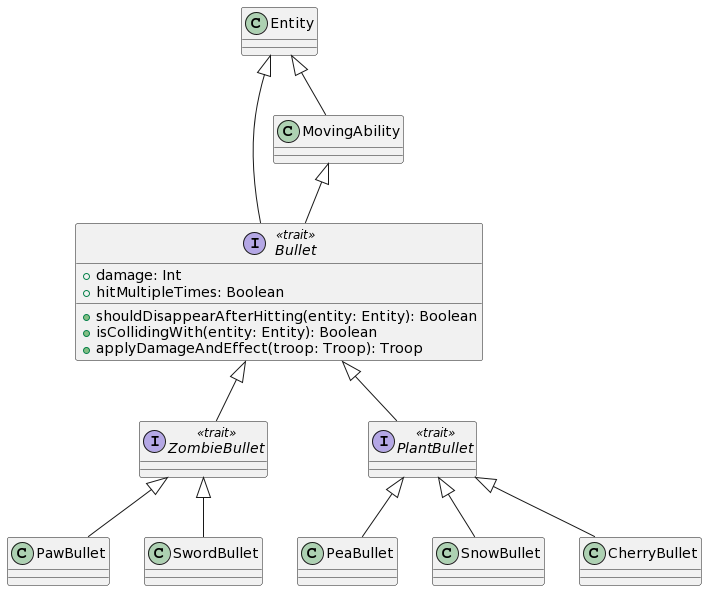
\includegraphics[width=1\linewidth]{images/model-bullet}
    \caption{Diagramma delle classi rappresentante i \texttt{ZombieBullet}.}
    \label{fig:class-bullet}
\end{figure}

Il model del \texttt{Bullet} è stato testato nella classe \texttt{BulletModelTest}.

\subsubsection{BulletActor}
Avendo adottando un'architettura ad attori, abbiamo pensato di incapsulare il comportamento
di ogni proiettile dentro un \texttt{BulletActor}. Quindi, in fase di creazione, ogni \texttt{Bullet} sarà associato ad un
\texttt{BulletActor} che ne definirà il comportamento.
Il \texttt{BulletActor} ha un solo Behaviour chiamato \texttt{moving}: risponde ai messaggi ricevuti dal \texttt{GameLoop}.

Come il \texttt{TroopActor}, ad ogni iterazione del \texttt{GameLoop} il \texttt{BulletActor} riceve un messaggio di \texttt{Update()} a seguito del quale:
\begin{enumerate}
    \item Aggiorna il proprio \texttt{Bullet}.
    \item Manda il suo \texttt{Bullet} aggiornato al \texttt{GameLoop}.
    \item Ricrea il proprio Behaviour con il \texttt{Bullet} aggiornato.
\end{enumerate}
Quando il \texttt{Bullet} collide con un'altra entità riceve un messaggio \texttt{Collision()} a seguito del quale:
\begin{enumerate}
    \item Crea il \texttt{Bullet} della propria \texttt{Troop}.
    \item Crea un \texttt{BulletActor} che controlla il \texttt{Bullet}.
    \item Notifica il \texttt{GameLoop} dell'avvenuta creazione con il messaggio \texttt{BulletSpawned()}.
\end{enumerate}
\newpage
Il comportamento del \texttt{BulletActor} viene mostrato nel seguente diagramma:
\begin{figure}[H]
    \centering
    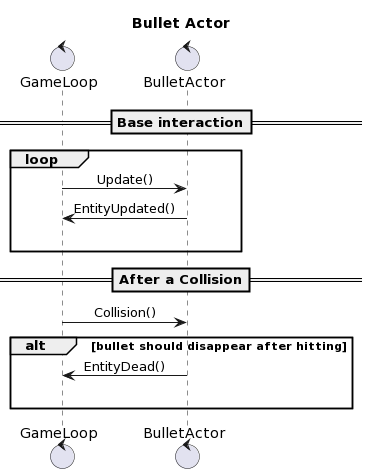
\includegraphics[width=0.8\linewidth]{images/bullet-actor.png}
    \caption{Diagramma di sequenza del Bullet Actor.}
\end{figure}

Il \texttt{BulletActor} è stato testato nella classe \texttt{BulletActorTest} utilizzando il framework \textbf{AkkaTest}.

\subsubsection{Zombie}
Gli \texttt{Zombie} rappresentano una delle entità fondamentali del gioco. In particolare, rappresentano i nemici che l'utente
deve cercare di eliminare attraverso il piazzamento delle piante nel campo di gioco.
Tutti gli \texttt{Zombie} sono in grado di muoversi orrizzontalmente nelle lane del campo di gioco con una certa velocità: pertanto
attraverso il meccanismo dei mixins il \texttt{trait Zombie} estende il \texttt{trait Troop} a cui aggiunge poi l' abilità \texttt{MovingAbility}.

Quando uno \texttt{Zombie} è colpito da un \texttt{SnowBullet} potrebbe essere rallentato, per questo motivo si è deciso di
mettere la velocità in ciascun costruttore per ciascun tipo di \texttt{Zombie} implementato.
In questo modo, seguendo un approccio funzionale e favorendo l'immutabilità delle istanze, quando lo \texttt{SnowBullet} collide con uno specifico \texttt{Zombie}
istanzierà nuovamente lo \texttt{Zombie} con la velocità aggiornata.
A tal proposito è stata implementata una val \texttt{slowVelocities} dentro all'object \texttt{ZombieDefaultValues}.

E' infatti nell'object \texttt{ZombieDefaultValue} che sono definite tutte le caratteristiche principali per ogni
tipo di \texttt{Zombie} implementato: stato iniziale e di default (\texttt{Moving}), vita iniziale,
il tipo \texttt{Bullet} a disposizione, la velocità di default, la velocità degli \texttt{Zombie} rallentati e un metodo per generare
la posizione iniziale degli \texttt{Zombie}.

Come mostrato nel diagramma delle classi degli \texttt{Zombie}, ogni classe che rappresenta uno \texttt{Zombie} deve estendere dal \texttt{trait Zombie}.

\begin{figure}[H]
    \centering
    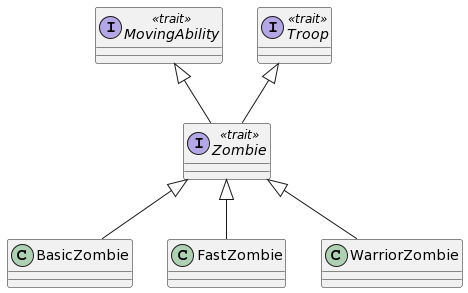
\includegraphics[width=1\linewidth]{images/model-zombie.png}
    \caption{Diagramma delle classi rappresentante gli \texttt{Zombie}.}
    \label{fig:class-zombie}
\end{figure}

Il comportamento degli \texttt{Zombie} è incapsulato nel \texttt{TroopActor} e il model degli \texttt{Zombie} è stato testato nella classe \texttt{ZombieModelTest}.

\section{Davide Alpi}
La mia responsabilità principale è stata l'implementazione della view del gioco.

Per prima cosa motiverò la mia scelta della libreria grafica (libGDX).
In seguito, descriverò il package "scalagdx", un layer che ho creato on top di libGDX per semplificarne e renderne più idiomatico l'utilizzo.
Infine, illustrerò l'interazione tra la view e l'ActorSystem, con seguente zoom sul ViewActor.


\subsection{Libreria grafica}
\label{sec:view}

Le librerie grafiche che ho valutato per lo sviluppo della parte di View sono state:
\begin{itemize}
    \item ScalaFX: la libreria più usata all'interno dell'ecosistema Scala per la creazione di interfacce grafiche
    \item Indigo: libreria Scala per la creazione di giochi
    \item libGDX: la libreria Java ad alto livello più usata per la creazione di giochi
\end{itemize}
Verrà scelta la tecnologia tenendo conto dei seguenti parametri:
\begin{itemize}
    \item Qualità della documentazione: La documentazione è completa e aggiornata? Gli esempi forniti compilano?
    \item Adozione: quanti progetti, commerciali e non, sono stati completati con questa tecnologia?
    \item Query results: numero di risultati di query google relative a diverse problematiche che gli sviluppatori tipicamente devono affrontare durante l'utilizzo della libreria.
    \item Funzionalità: quanto permette di fare? Quanto è vasta e flessibile l'API fornita?
\end{itemize}

\subsubsection{Indigo}
Indigo è stata subito scartata perchè nessun progetto commerciale è ancora stato completato con il suo utilizzo (livello di adozione troppo basso). Anche gli altri parametri non raggiungono livelli soddisfacenti.

\subsubsection{ScalaFX}
ScalaFX, pur essendo la libreria Scala più utilizzata per la creazione di interfacce grafiche, rimane una libreria Scala, e pertanto il suo grado di adozione è limitato.
La documentazione è molto scarna e alcuni esempi contenuti non buildano.

\subsubsection{libGDX - scelta finale}
Una miriade di progetti commerciali sono stati portati avanti con libGDX. La sua API nel corso degli ultimi 5 anni ha subito poche sostanziali modifiche, evidenziando un importante grado di maturità raggiunto. Essendo una libreria Java, il numero di query result è esponenzialmente maggiore rispetto alle altre scelte.

Da un punto di vista commerciale, libGDX è la scelta migliore.
Anche da un punto di vista di ricerca, è interessante capire come libGDX può essere inserito all'interno di un progetto Scala in maniera idiomatica. Si sfrutta anche la possibilità di Scala di accedere all'intero ecosistema Java. Per questa serie di motivazioni, ho scelto libGDX come libreria grafica.

\subsection{scalagdx}
Durante l'implementazione delle diverse schermate del gioco, per evitare boilerplate code e per rendere il codice più idiomatico, ho sentito la necessità di creare il package scalagdx. Di seguito ne illustro alcuni object salienti.

\subsubsection{Screen}
libGDX fornisce un'API che permette di definire in maniera piuttosto imperativa il codice da "agganciare" all'esecuzione di alcuni \textit{lifecylcle methods} delle schermate di gioco (\textit{ScreenAdapter}).
Un esempio è il metodo \textit{render}, metodo dello ScreenAdapter che verrà chiamato dal motore grafico ad ogni frame. Effettuandone l'override, è possibile quindi definire cosa disegnare a schermo ciascun frame. L'implementazione di diversi ScreenAdapter è tediosa, error-prone, e richiede una grande quantità di boilerplate code.

Con \textit{scalagdx.Screen.ScreenBehavior} ho voluto risolvere questo problema, fornendo un'API per definire in maniera più dichiarativa gli elementi che dovranno apparire a schermo. Lo \textit{ScreenBehavior} si basa anche sui concetti di \textit{Drawable} e \textit{Writable}, che modellano rispettivamente delle immagini e delle scritte unitamente ai loro boundaries all'interno del viewport.

\begin{lstlisting}[language=Scala, label=code:screen-behavior, caption=trait ScreenBehavior]
  trait ScreenBehavior:
    def drawables: Seq[Drawable]
    def writables: Seq[Writable]
    def actors: Seq[Actor]
    def onScreenTouch: Vector2 => Unit
    def viewport: Viewport
\end{lstlisting}

\begin{figure}[H]
    \centering
    \caption{ScreenBehavior's promise of execution}
    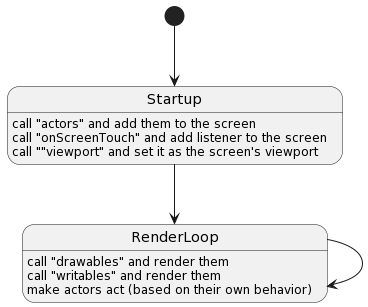
\includegraphics[width=0.8\linewidth]{images/screen-behavior.png}
    \label{ScreenBehavior}
\end{figure}


Lo ScreenBehavior può essere poi usato per costruire un BasicScreen, che implementa ScreenAdapter. Lo ScreenBehavior può anche essere convertito implicitamente in BasicScreen grazie al meccanismo delle given conversion.


\subsubsection{Clickable}
Il mio obiettivo era attuare il pattern \textbf{pimp my library} per aggiungere un metodo \textit{onTouchDown} e \textit{onTouchUp} alle classi di libGDX \textit{Actor} e \textit{Stage}.
Entrambi implementano il metodo "addListener" (con la stessa signature), ma non hanno sfortunatamente interfacce comuni da poter "pimpare" (con extension method ad esempio).
Una soluzione sarebbe stata implementare extension methods per entrambe le classi per implementare i due metodi di cui sopra per entrambe le classi. Questo avrebbe portato però alla duplicazione del codice.

La soluzione adottata è stata la seguente:

\begin{lstlisting}[language=Scala, label=code:clickable, caption=trait Clickable]
  trait Clickable:
    protected def addListener(cl: EventListener): Boolean
    def onTouchDown(f: Vector2 => Unit): Unit = addListener(new ClickListener :
      override def touchDown(event: InputEvent, x: Float, y: Float, pointerId: Int, buttonId: Int): Boolean =
        super.touchDown(event, x, y, pointerId, buttonId)
        f(Vector2(x, y))
        true
    )
    def onTouchUp(f: () => Unit): Unit = addListener(new ClickListener :
      override def touchUp(event: InputEvent, x: Float, y: Float, pointerId: Int, buttonId: Int): Unit =
        super.touchUp(event, x, y, pointerId, buttonId)
        f()
    )
    
  given Conversion[Actor, Clickable] = actor => new Clickable :
    export actor.addListener

  given Conversion[Stage, Clickable] = stage => new Clickable :
    export stage.addListener
\end{lstlisting}

Il trait Clickable implementa le funzionalità aggiuntive in comune tra tutte le classi che implementano \textit{addListener} (in questo caso \textit{Actor} e \textit{Stage}).

\subsubsection{ImageButton builder}
Per semplificare l'istanziamento di ImageButton, e ridurre la necessità di boilerplate code, ho realizzato il seguente builder.

\begin{lstlisting}[language=Scala, label=code:image-buttons, caption=Builder pattern per ImageButtons]

object ImageButtons:
  case class ImageButtonBuilder private[ImageButtons](source: Texture|ImageButtonStyle, bounds: Rectangle = Rectangle(0, 0, 0, 0)):
    def withBounds(x: Float, y: Float, width: Float, height: Float): ImageButtonBuilder = copy(bounds = Rectangle(x, y, width, height))

    def build: ImageButton =
      val button = source match
        case t: Texture => ImageButton(TextureRegionDrawable(t))
        case s: ImageButtonStyle => ImageButton(s)
      button.setBounds(bounds.x, bounds.y, bounds.width, bounds.height)
      button.setTransform(true)
      button

  def withSource(source: Texture|ImageButtonStyle): ImageButtonBuilder = ImageButtonBuilder(source)

  given Conversion[ImageButtonBuilder, ImageButton] = _.build
  
\end{lstlisting}

Grazie alla given conversion, è possibile evitare la chiamata finale al \textit{build()} e rendere così il suo utilizzo più fluente:

\begin{lstlisting}[language=Scala, label=code:image-buttons-example, caption=Esempio di creazione di un ImageButton con e senza given conversion abilitata]

val source: Texture = ???

ImageButtons.withSource(source).withBounds(0,0,0,0).build()

import ImageButtons.given

ImageButtons withSource source withBounds (0,0,0,0)

\end{lstlisting}

Questo builder pattern potrebbe essere implementato anche per molte altre classi di libGDX che si intendono usare, seguendo lo stesso schema.
Nel caso degli ImageButton, una source è obbligatoria per la creazione dell'oggetto, ma in caso il builder non richieda parametri obbligatori basta cambiare il metodo \textit{withSource(...)} in un generico \textit{builder}.


\subsection{Game}

\subsubsection{Lancio dell'applicazione}
Una volta sviluppato il \textit{core} di un'applicazione con libGDX, occorre definire un \textit{main} ad hoc per ciascuna piattaforma che si intende supportare. Ho creato quindi un launcher con LWJGL3 per supportare i dispositivi desktop.

Al launcher LWJGL3 deve essere fornita una particolare classe di libGDX. Ho implementato quindi un'estensione di questa classe, "\textbf{Game}", che rappresenta l'entry point del \textit{core} della nostra applicazione.

Il Game agisce da top level controller dell'applicazione, occupandosi di avviare l'ActorSystem ogni volta che viene avviata una nuova partita e cambiando schermata quando richiesto.

\subsubsection{Interazione tra Game e ActorSystem}
Di seguito le interazioni tra il \textbf{Game} e l'\textbf{ActorSystem} (che contiene, tra gli altri attori, il ViewActor).
Sono mostrate anche le tre schermate di gioco, implementate con \textit{MainMenuScreen}, \textit{GameScreen} e \textit{GameOverScreen}.


\begin{figure}[H]
    \centering
    \caption{Interazioni di lancio applicazione, inizio partita e fine partita}
    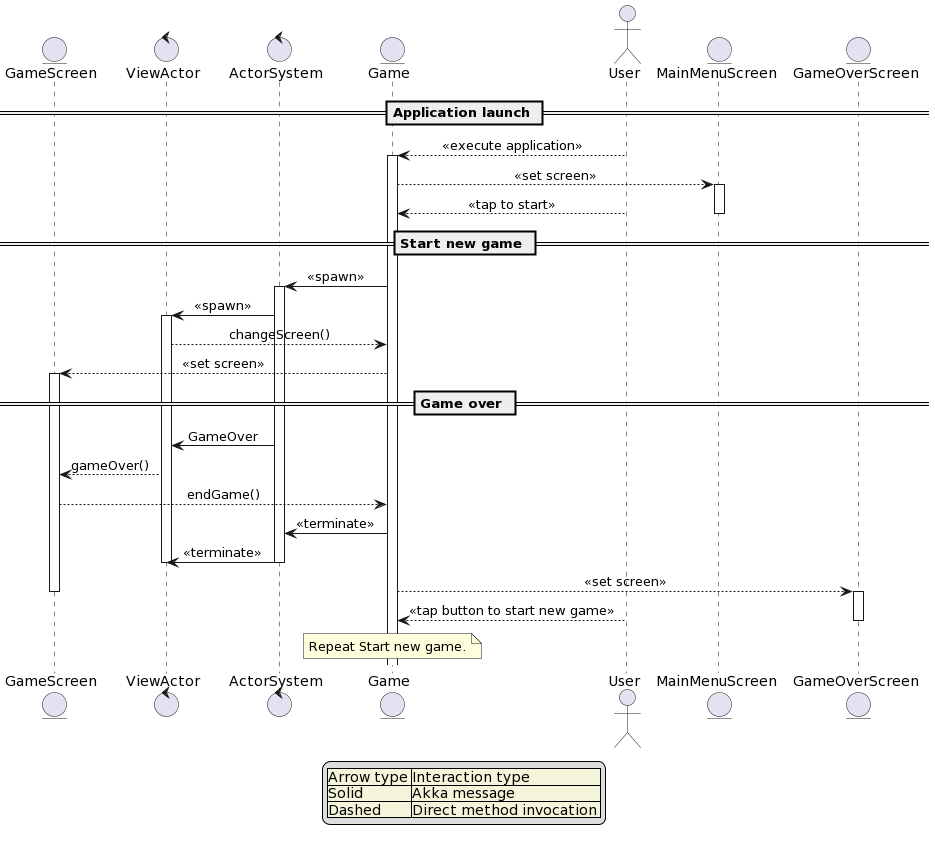
\includegraphics[width=0.8\linewidth]{images/actors-game-interaction.png}
    \label{ScreenBehavior}
\end{figure}


\subsubsection{ViewActor}
Il ViewActor rappresenta la parte di View dell'ActorSystem, come illustrato nel capitolo relativo al Design di Dettaglio. Il seguente diagramma di sequenza mostra come ho gestito le interazioni tra esso e il GameScreen.

\begin{figure}[H]
    \centering
    \caption{ViewActor message exchange during game}
    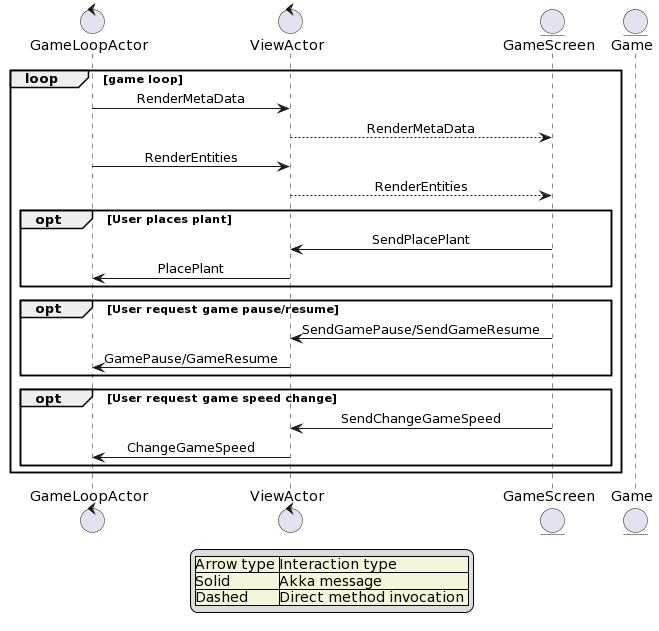
\includegraphics[width=0.8\linewidth]{images/view-actor.png}
    \label{ScreenBehavior}
\end{figure}


    \newpage
\section{Retrospettiva}
I vari documenti relativi alle singole iterazioni (sprint), inclusi quelli di planning e retrospettiva, sono reperibili all'ultima release nel file \texttt{backlog.pdf}.


In questa ultima sezione vogliamo discutere a posteriori del processo di sviluppo, della sua evoluzione, e dei lati positivi e negativi riscontrati.

\subsection{Processo di sviluppo}
\subsubsection{Daily Meeting}
Durante il primo e secondo sprint abbiamo adottato un processo che includeva daily meeting. Durante queste riunioni veniva anche redatto un verbale. Dal terzo sprint a causa della difficoltà dei membri del team nell'accordarsi per un orario fisso abbiamo gradualmente rimosso questo appuntamento. Essere riusciti a mantenere inizialmente i daily sprint ha facilitato il processo di design incrementale. Lo svantaggio della loro rimozione è stata una maggiore difficoltà nel mantenere l'allineamento dei membri del team su di una visione d'insieme del processo di sviluppo.

\subsubsection{Pull request vs Pair programming}
Utilizzando il meccanismo delle pull request, ci siamo resi conto di quanto questo sia utile per mantenere traccia di tutte le decisioni e per favorire il lavoro asincrono.
La tendenza del gruppo è stata quella di cooperare prevalentemente tramite chiamata su Teams durante lo sviluppo delle feature. In questi casi si è perso il vantaggio delle pull request, ma si è ottenuta una maggiore agilità.
Crediamo che il team abbia raggiunto il giusto compromesso da questo punto di vista, utilizzando il meccanismo delle pull request per le feature più corpose e significative, e lasciando alla collaborazione vocale/pair programming il resto.

Altro vantaggio dell'ampia collaborazione vocale non citato: sopperire alla distanza fisica del team (che ha lavorato diviso tra Italia e Svezia).

\subsubsection{Tools}
Il processo di sviluppo avrebbe giovato di una maggiore integrazione tra product backlog e Trello. L'elemento di viscosità riscontrato è stato il dover riscrivere i task con relativa descrizione in entrambi i posti.



\subsection{Commenti finali}
Il sentimento comune di tutti i componenti del gruppo è che Scala si adatta molto bene ad una metodologia di sviluppo Agile, grazie all'enorme flessibilità derivante dall'arsenale di meccanismi che mette a disposizione.

Nel complesso, siamo soddisfatti di quello che è stato prodotto. Il gruppo ha terminato il monte ore assegnato al progetto ma sarebbe entusiasta di proseguire lo sviluppo di feature opzionali.

\end{document}
